\documentclass[a4paper, 11pt, dvipdfmx]{jsarticle}
\usepackage[utf8]{inputenc}

\usepackage{graphicx}
\usepackage{hyperref}
\usepackage{bookmark}
\usepackage{fontawesome5}
\usepackage{tcolorbox}
\tcbuselibrary{breakable, listingsutf8}

\usepackage{geometry}
\geometry{left=20mm,right=20mm,top=20mm,bottom=20mm}

\usepackage{chngcntr}
\usepackage{listings}
\usepackage{float} % 追加

\tcbset{
  colframe=black,
  colback=gray!20,
  fonttitle=\bfseries,
  sharp corners,
  breakable = true,
  boxrule=0.5mm,
  left=1mm,
  right=1mm,
  top=1mm,
  bottom=1mm,
}
\tcbset{
  comandstyle/.style={
    colframe=black,
    colback=black,
    coltitle=white,
    coltext=white,
    fonttitle=\ttfamily,
    sharp corners = all,
    breakable = true,
    title=コマンド,
  },
  yellow/.style={
    colframe=yellow,
    colback=yellow!10,
    coltitle=black,
    fonttitle=\bfseries,
    title={\faIcon{exclamation-triangle} 注意}
  },
  blue/.style={
    colframe=blue,
    colback=blue!10,
    coltitle=white,
    fonttitle=\bfseries,
    title={\faIcon{info-circle} 情報}
  },
  green/.style={
    colframe=green!80!black,
    colback=green!10,
    coltitle=white,
    fonttitle=\bfseries,
    title={\faIcon{bookmark} 補足説明}
  },
}

\newtcolorbox{commandbox}[2][]{comandstyle, title=#2, #1}

\usepackage{titlesec}
\usepackage{tocloft}

% セクション番号の変更
\titleformat{\section}{\normalfont\Large\bfseries}{\thesection 章}{1em}{}
\titleformat{\subsection}{\normalfont\large\bfseries}{\thesection.\arabic{subsection}}{1em}{}
\titleformat{\subsubsection}{\normalfont\normalsize\bfseries}{\thesection.\arabic{subsection}.\arabic{subsubsection}}{1em}{}

\begin{document}

\title{Linuxサーバー構築手順書}
\author{大阪公立大学工業高等専門学校\\
3年 知能情報コース 5番\\
}
\date{\today}
\maketitle\thispagestyle{empty}
\newpage
\tableofcontents

\newpage
\setcounter{section}{-1}

\section{はじめに}

\section{Linuxについて}
\subsection{ファイルやディレクトリ構造について}
Linuxではディレクトリ構造がWindowsとは異なる。
\subsubsection{ファイルの種類}
  Linuxで扱われるファイルは以下のように分類される。
  \begin{itemize}
    \item ファイル     :テキストファイルとバイナリファイル
    \item リンクファイル :シンボリックリンクとハードリンク
    \item 特殊ファイル  :デバイスファイルや隠しファイル
    \item ディレクトリ  :ファイルを集約するためのWindowsでいうフォルダ
  \end{itemize}
  拡張子はWindowsにおいてはアプリケーションの起動に紐づけられていたが、Linuxでは単なるファイル名の一部として認識される。\\
  Linuxではデバイスファイルがあり、これはハードウェアをファイルとして扱うためのものである。\\

  \subsubsection{ディレクトリ構造}
  Linuxのディレクトリ構造は/(ルート)を起点として以下のディレクトリが主に挙げられる。それらをある程度理解しておくことで各種設定などの変更の際に便利である。\\
  \begin{table}[h]
    \centering
    \begin{tabular}{|l|l|}
      \hline
      ディレクトリ & 説明 \\ \hline
      /root & システム管理者のホームディレクトリ \\ \hline
      /home & 一般ユーザーのホームディレクトリ \\ \hline
      /bin & 一般ユーザーでも実行可能なコマンドが含まれるディレクトリ \\ \hline
      /sbin & sudo権限またはroot権限が必要なコマンドが含まれるディレクトリ \\ \hline
      /media & USBメモリや外付けHDDなどのデバイスがマウントされるディレクトリ \\ \hline
      /etc & システムの設定ファイルが含まれるディレクトリ \\ \hline
      /usr & システム全体で共有されるアプリケーション、ライブラリ、ドキュメントなどが保存されるディレクトリ \\ \hline
      /lib & ライブラリが保存されるディレクトリ \\ \hline
      /proc & カーネルやプロセスに関する情報が保存されるディレクトリ \\ \hline
      /tmp & 一時ファイルが保存されるディレクトリ \\ \hline
      /var & 変化するデータが保存されるディレクトリ、ログファイルやデータベースなど \\ \hline
    \end{tabular}
    \caption{主要なディレクトリとその説明}
    \label{tab:directories}
  \end{table}
  表\ref{tab:directories}に主要なディレクトリとその説明を示す。


\section{Ubuntuインストール}
\subsection{インストールメディアの準備}
  \begin{enumerate}
    \item UbuntuのISOファイルをダウンロード
    \begin{tcolorbox}[blue]
      Ubuntu を入手する \href{https://releases.ubuntu.com/20.04/}{\texttt{https://releases.ubuntu.com/20.04/}}\\
      Ubuntu Desktop 日本語 Remixのダウンロード \href{https://www.ubuntulinux.jp/download/ja-remix}{\texttt{https://www.ubuntulinux.jp/download/ja-remix}}
    \end{tcolorbox}
    \item Rufusをダウンロード
    \begin{tcolorbox}[blue]
      Rufusを入手する \href{https://rufus.ie/ja/}{\texttt{https://rufus.ie/ja/}}
    \end{tcolorbox}
    \item Rufusを起動し、デバイス、ブート選択、イメージ選択を行う\\
    デバイスにはインストールメディアとするためのUSBを選択する。\\
    ブート選択では、先ほどダウンロードしたISOファイルを選択する。\\
    パーティション構成は一般的にはMBRでよい。ただし、Gatewayの場合はGPTを選択する。その他の設定はデフォルトのままでよい。
      \begin{tcolorbox}[yellow]
        デバイスを選択する際は注意が必要である。間違えるとPCや外部ストレージのデータが消える可能性があるため、注意が必要である。
      \end{tcolorbox}
    \item スタートをクリックし、書き込みを開始する
  \end{enumerate}

\subsection{Boot Modeの変更}
  \begin{enumerate}
    \item 電源をつけF2を連打しBIOS画面を表示
    \item Securityに移動しSupervisor Passwordを設定
    \item Bootに移動しBoot ModeをLegacyに変更
    \item F10で保存して再起動
    \item F2を連打しBIOS画面を表示
    \item Bootに移動しBoot Priorityを変更しインストールメディアが入るものを選択
    \item Boot ModeをUEFIに変更
    \item SecureBootをDisableに変更
    \item F10で保存して再起動
  \end{enumerate}
\subsection{Ubuntuのインストール}
  \begin{enumerate}
    \item 再起動後自動的にBoot Menuが表示される
    \item Try or Install Ubuntuを選択
    % \item 以下Ubuntuのインストールを書く ★
    \item インストールの種類を選択
    \item インストール先を選択
    \item キーボードレイアウトを選択
    \item ユーザー情報を入力
    \item インストールが完了したら再起動
  \end{enumerate}
\subsection{インストール後の再起動}
  \begin{enumerate}
    \item 再起動時にBiosに入る
    \item Bootに移動しBoot Priorityを変更しインストールしたディスクを1番目にする
    \item SecureをEnableに変更
    \item Securityに移動しErase all Secure Boot Settingを選択し、Boot設定を削除
    \item Select an UEFI file as trusted for executingを選択
    \item EMMC \textgreater EFI \textgreater Ubuntu \textgreater shimx64.efiを選択
    \item Boot名を入力し、Enter
    \item Bootに移動しSecure BootをDisableに変更
    \item Securityに移動しSupervisor Passwordを削除
    \item F10で保存して再起動
    \item ログイン画面になったら成功
  \end{enumerate}

\section{Ubuntuの各種設定・インストール}
Ubuntu(Linux)はWindowsなどと同様に様々な設定が可能である。以下にはその一部を示すが、適宜自分にあったUbuntu環境を構築することが望ましい。練習ついでにいろいろな物を入れてみるとよい。
\subsection{日本語入力}
  Ubuntuではデフォルトでキーボードによる日本語入力は対応していない。そのため、以下の手順で日本語入力を可能にする。なお日本語入力には一般に「Mozc」が使用されることが多い。
  \begin{enumerate}
    \item ターミナルを開く
    \item 以下のコマンドを実行
    \begin{commandbox}{コマンド}
      \verb|$ sudo apt update|\\
      \verb|$ sudo apt install ibus-mozc|
    \end{commandbox}
    \item 設定 \textgreater キーボード \textgreater 入力ソース \textgreater 日本語(Mozc)を追加
    \item Windowsキー + Spaceで日本語入力が可能になる\\
    なお、右上にある「A」をクリックすることで入力ソースを切り替えることができる。
  \end{enumerate}

\subsection{Vimのインストール}
  VimはLinux環境で使用されるテキストエディタであり、非常に高機能である。特徴として、ターミナル上で操作するため、マウスを使わずに編集を行う。本手手順書ではsudo権限(後の章にて解説)の必要なファイルの編集などで使用する。標準で搭載されている場合もある。
  \begin{enumerate}
    \item ターミナルを開く
    \item 以下のコマンドを実行
    \begin{commandbox}{コマンド}
      \verb|$ sudo apt update|\\
      \verb|$ sudo apt install vim|
    \end{commandbox}
    \item インストールが完了したら、以下コマンドを実行しインストールされているか確認
    \begin{commandbox}{コマンド}
      \verb|$ vim --version|
    \end{commandbox}
  \end{enumerate}

\subsection{VSCodeのインストール}
  VSCodeはMicrosoftが提供するオープンソースのコードエディタであり、非常に高機能である。特徴として、拡張機能を追加することで、様々な言語に対応することができる。また、リモート開発機能を使用することで、リモートサーバー上での開発も可能である。
  \begin{enumerate}
    \item \href{https://code.visualstudio.com/}{\texttt{https://code.visualstudio.com/}}にアクセスし、ダウンロード
    \item ダウンロードしたファイルを開く
    \item インストールを開始
    \item インストールが完了したら、VSCodeを起動
  \end{enumerate}

\subsection{slのインストール(お遊び)} 
  slは、タイプミスでよく入力される「ls」コマンドを実行すると、蒸気機関車が走るアニメーションが表示されるコマンドである。インストールの練習として入れてみるとよい。
  \begin{enumerate}
    \item ターミナルを開く
    \item 以下のコマンドを実行
    \begin{commandbox}{コマンド}
      \verb|$ sudo apt update|\\
      \verb|$ sudo apt install sl|
    \end{commandbox}
    \item 以下のコマンドを実行
    \begin{commandbox}{コマンド}
      \verb|$ sl|
    \end{commandbox}
  \end{enumerate}
  \begin{figure}[H]
    \centering
    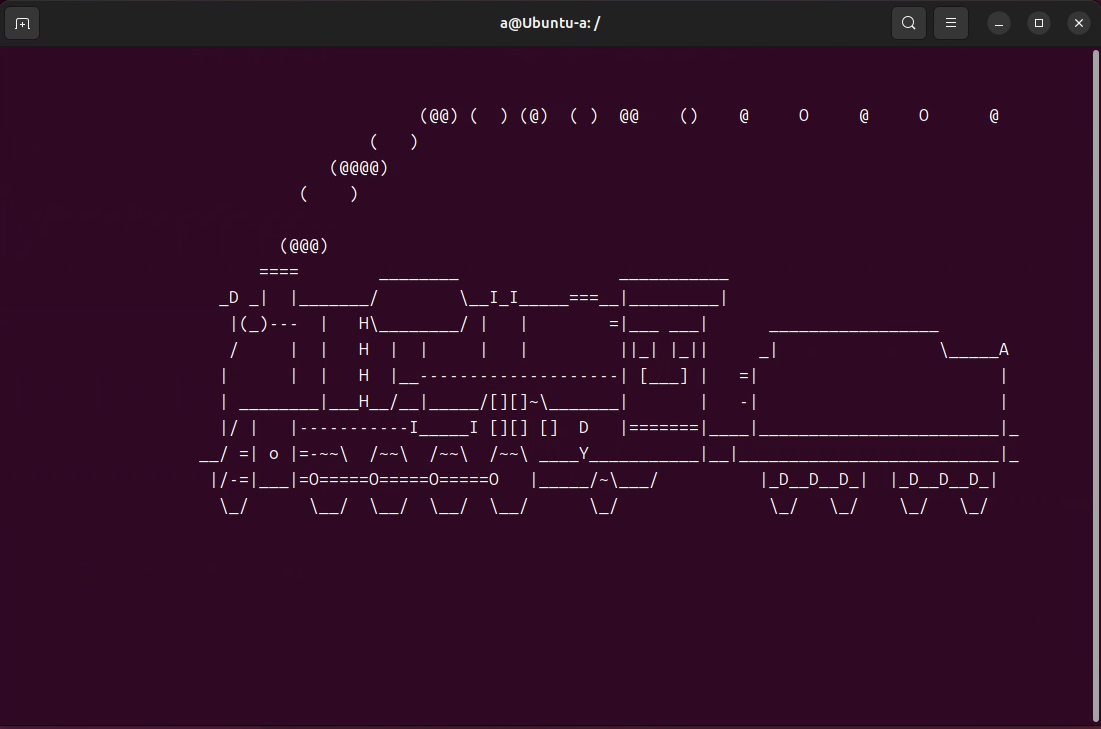
\includegraphics[width=0.5\textwidth]{images/linux-server/3_4-sl.png}
    \caption{slの実行結果}
    \label{fig:sl}
  \end{figure}
  実行時にオプションがあるので、気が向いたら調べて遊んでみるとよい。

\subsection{cmatrixのインストール(お遊び)}
  cmatrixは、映画「マトリックス」に登場するコードのような文字列が画面上を流れるアニメーションを表示するコマンドである。ハッカーみたいになれるのでなりたい人は入れるとよい。
  \begin{enumerate}
    \item ターミナルを開く
    \item 以下のコマンドを実行
    \begin{commandbox}{コマンド}
      \verb|$ sudo apt update|\\
      \verb|$ sudo apt install cmatrix|
    \end{commandbox}
    \item 以下のコマンドを実行
    \begin{commandbox}{コマンド}
      \verb|$ cmatrix|
    \end{commandbox}
  \end{enumerate}
  \begin{figure}[H]
    \centering
    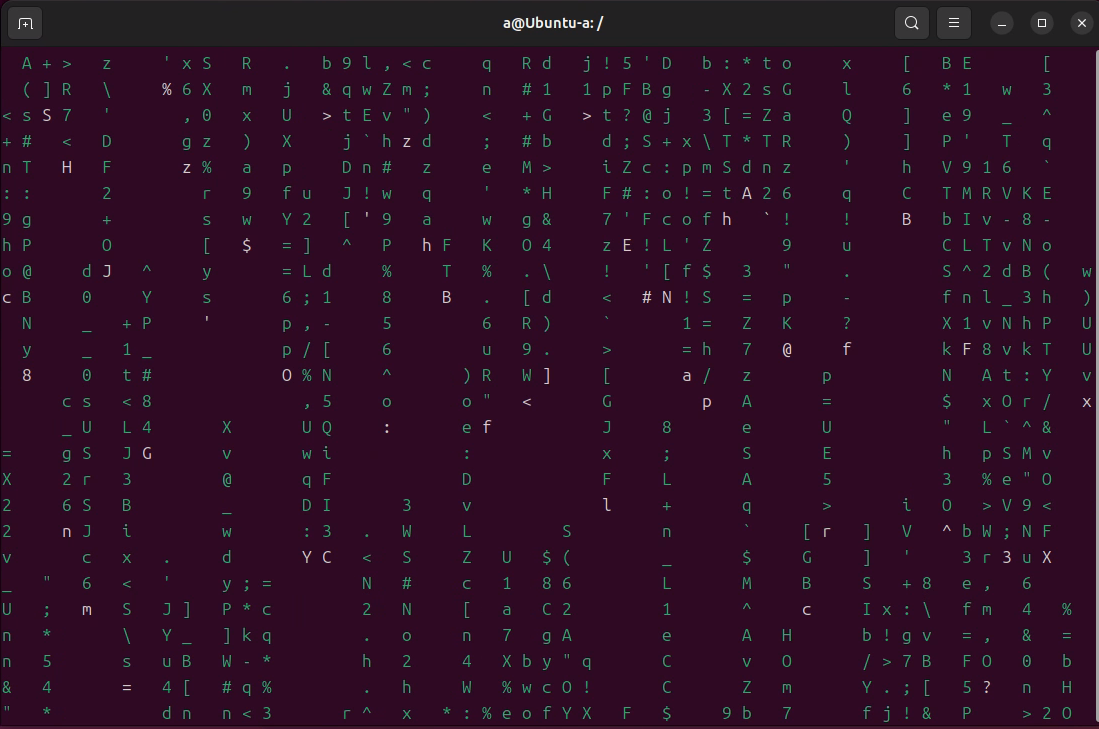
\includegraphics[width=0.5\textwidth]{images/linux-server/3_5-cmatrix.png}
    \caption{cmatrixの実行結果}
    \label{fig:cmatrix}
  \end{figure}

\section{Linuxの基本コマンド}

\section{パーミッション}

\section{環境変数}

\section{テキストエディタ}

\section{ネットワーク設定}

\section{ユーザー管理}

\section{SSH}

\section{基本的なサーバー管理}

\section{Webサーバーの構築}

\section{Dockerを使用した環境構築や運用}

\section{終わりに}






\end{document}